\documentclass{cubeamer}

\usepackage{trimclip}
\usepackage{wrapfig}
\usepackage{graphicx}
\usepackage{caption}
\usepackage{subcaption}
\usepackage{tikz}
\usetikzlibrary{positioning}
\usetikzlibrary{arrows.meta}
\usetikzlibrary{arrows,shapes,quotes}
\usepackage{amsmath,amsfonts}

\title{Automated Deduction for Intuitionistic Logic via Embedding into Classical Logic}
\subtitle{Defensio}
\author[Alexander Pluska]{Alexander Pluska}
\date{\today} % or whatever the date you are presenting in is
\institute[University of Vienna]{University of Vienna}
% \copyrightnotice{Published by the American Institute of Aeronautics and Astronautics, Inc., with permission}

\begin{document}
	
	\maketitle
	
	\cutoc
	
	\section{Background}
	
	\begin{frame}{Automated Deduction}
			\begin{figure}[!tbp]
				\centering
				\begin{subfigure}[b]{0.35\textwidth}
					\begin{center}
						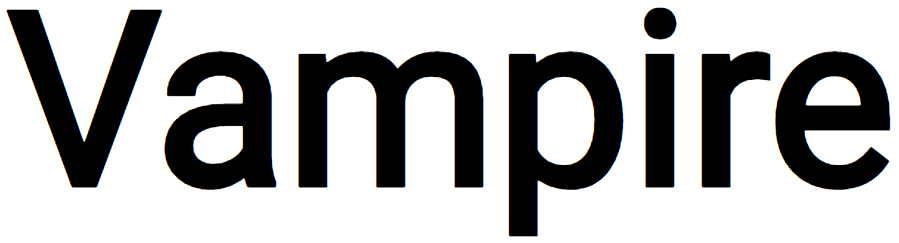
\includegraphics[width=\textwidth]{Vampire.png}
						\begin{subfigure}[b]{0.4\textwidth}
							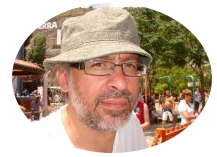
\includegraphics[height=0.2\textheight]{Voronkov.png}
						\end{subfigure}
						\hfill
						\begin{subfigure}[b]{0.4\textwidth}
							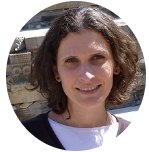
\includegraphics[height=0.2\textheight]{Kovacs.png}
						\end{subfigure}
						\caption{Andrei Voronkov \& Laura Kovács}
					\end{center}
				\end{subfigure}
				\hfill
				\begin{subfigure}[b]{0.6\textwidth}
					\includegraphics[width=\textwidth]{CASC.png}
					\caption{CASC-28 Results}
				\end{subfigure}
			\end{figure}
	\end{frame}
	
	\begin{frame}{Intuitionistic Logic}
		\begin{figure}[!tbp]
			\centering
			\begin{subfigure}[][][t]{0.6\textwidth}
				\begin{itemize}
					\item Motivation:
					\begin{itemize}
						\item Mathematical Constructivism.
						\item Curry-Howard-Correspondence.
					\end{itemize}
					\item Not intuitionistically valid:
					$$\neg\neg A\to A\hspace*{1cm} \forall x\neg\neg A(x)\to \neg\neg\forall x A(x)$$
				\end{itemize}
			\end{subfigure}
			\hfill
			\begin{subfigure}[]{0.3\textwidth}
				\centering
				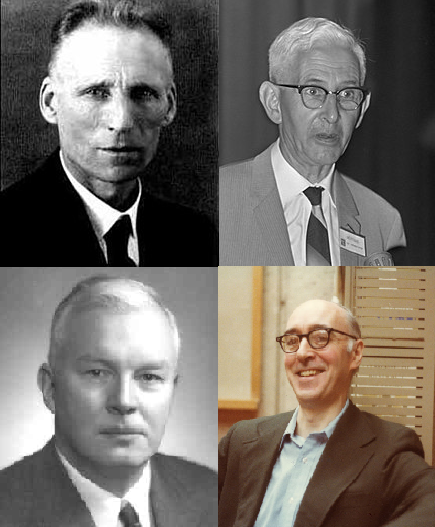
\includegraphics[width=0.9\textwidth]{logicians.png}
				\caption{L. E. J. Brouwer, A. Heyting, H. B. Curry, W. A. Howard}
			\end{subfigure}
		\end{figure}
	\end{frame}

	\begin{frame}{Kripke Semantics}
		\begin{definition}
			A \textit{Kripke structure} $\mathcal K = (W, (v_w)_{w\in W})$ consists of a partially ordered set $W$ of worlds and a family of valuations $(v_w)_{w\in W}$ such that for $u\leq w$ we have $v_u(A)\leq v_w(A)$ for every propositional variable $A$. We define a model relation between worlds $u$ and formulas as follow:
			\begin{itemize}
				\item $u\not\models \bot$
				\item $u\models A$ iff $v_u(A) = 1$ for each propositional variable $A$.
				\item $u\models \varphi\wedge\psi$ iff $v\models\varphi$ and $v\models\psi$.
				\item $u\models\varphi\vee\psi$ iff $v\models\varphi$ or $v\models\psi$.
				\item $u\models\varphi\to \psi$ if for all $w\geq u$ we have $w\not\models\varphi$ or $w\models\psi$.
			\end{itemize}
		\end{definition}
	\end{frame}
	
	\begin{frame}{Kripke Semantics - Example}
			\begin{figure}[!tbp]
			\centering
			\begin{subfigure}[][][t]{0.3\textwidth}
				\centering
					$A\vee\neg A\:\approx$ ``$A$ or never $A$''\vspace*{1cm}
					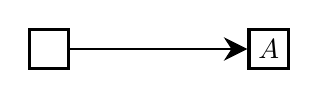
\begin{tikzpicture}[squarednode/.style={rectangle, draw, very thick, minimum size=5mm}]
						\node (center) {};
						\node[squarednode]      (left)   [left=of center] {};
						\node[squarednode]      (right)       	[right=of center] {$A$};
						\draw[-{Stealth[length=3mm, width=3mm]}] (left.east) -- (right.west);	
					\end{tikzpicture}
				\caption{Counter-model $A\vee\neg A$}
			\end{subfigure}
			\hfill
		\begin{subfigure}[][][t]{0.6\textwidth}
			\centering
			$\forall x\neg\neg A(x)\to \neg\neg\forall x A(x)\:\approx$ ``for all $x$ eventually $A(x)$ implies eventually for all $x$ $A(x)$''\vspace*{1cm}
			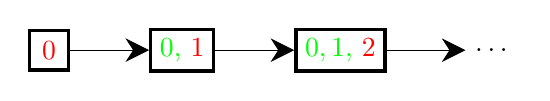
\begin{tikzpicture}[squarednode/.style={rectangle, draw, very thick, minimum size=5mm}]
				\node[squarednode]  (0) {\color{red}$0$};
				\node[squarednode]      (1)   [right=of 0] {\color{green}$0$, \color{red}$1$};
				\node[squarednode]      (2)       	[right=of 1] {\color{green}$0, 1$, \color{red}$2$};
				\node   (3)       	[right=of 2] {\dots};
				\draw[-{Stealth[length=3mm, width=3mm]}] (0.east) -- (1.west);	
				\draw[-{Stealth[length=3mm, width=3mm]}] (1.east) -- (2.west);
				\draw[-{Stealth[length=3mm, width=3mm]}] (2.east) -- (3.west);	
			\end{tikzpicture}
			\caption{Counter-model $\forall x\neg\neg A(x)\to \neg\neg\forall x A(x)$}
		\end{subfigure}
		\end{figure}
	\end{frame}
	
	\begin{frame}{Automated Deduction for Intuitionistic Logic}
		\begin{figure}
			\begin{subfigure}{0.49\textwidth}
				\centering
				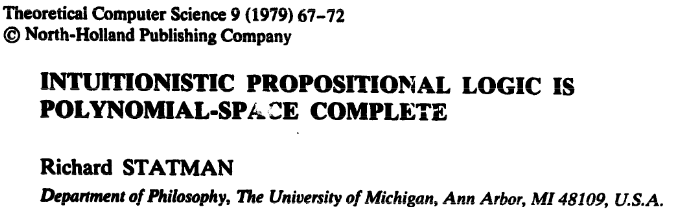
\includegraphics[width=\textwidth]{statman.png}
			\end{subfigure}
			\begin{subfigure}{0.49\textwidth}
				\centering
				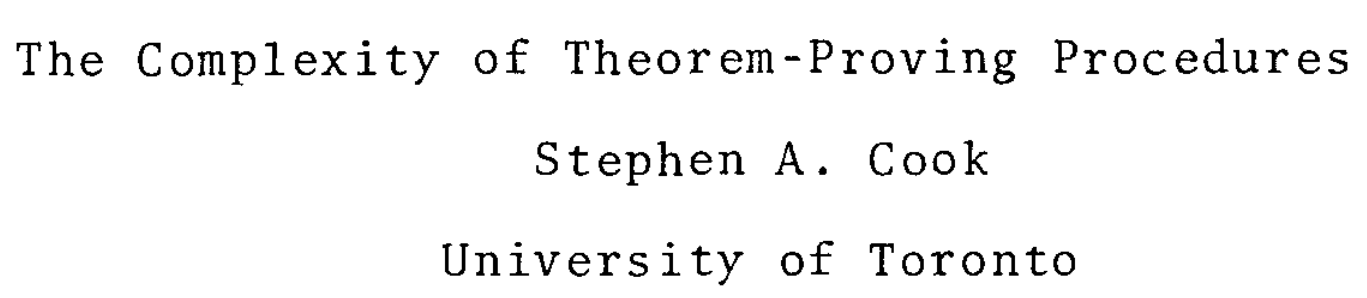
\includegraphics[width=\textwidth]{cook.png}
			\end{subfigure}
		\begin{subfigure}[b]{0.49\textwidth}
			\centering
				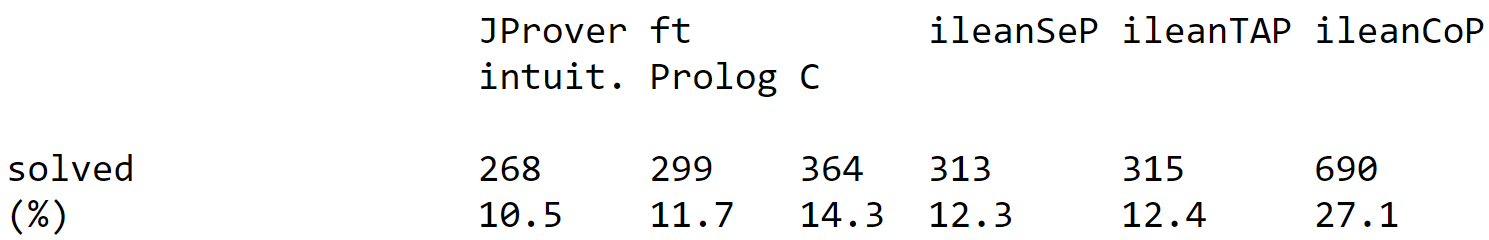
\includegraphics[width=\textwidth]{iltp.png}
			\caption{ILTP benchmark}
		\end{subfigure}
		\begin{subfigure}[b]{0.49\textwidth}
			\includegraphics[width=0.9\textwidth]{CASC.png}
			\caption{CASC-28 Results}
		\end{subfigure}
		\end{figure}
	\end{frame}
	
	\begin{frame}{Existing approaches}
		\begin{figure}
			\begin{subfigure}{0.49\textwidth}
				\centering
				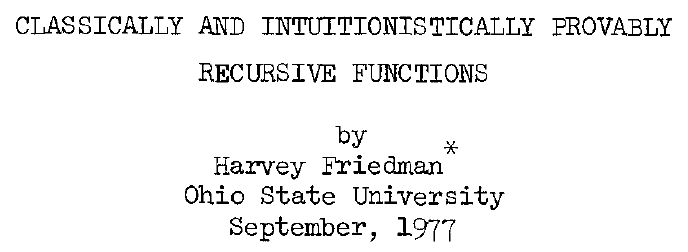
\includegraphics[width=\textwidth]{friedman.png}
			\end{subfigure}
			\begin{subfigure}{0.49\textwidth}
				\centering
				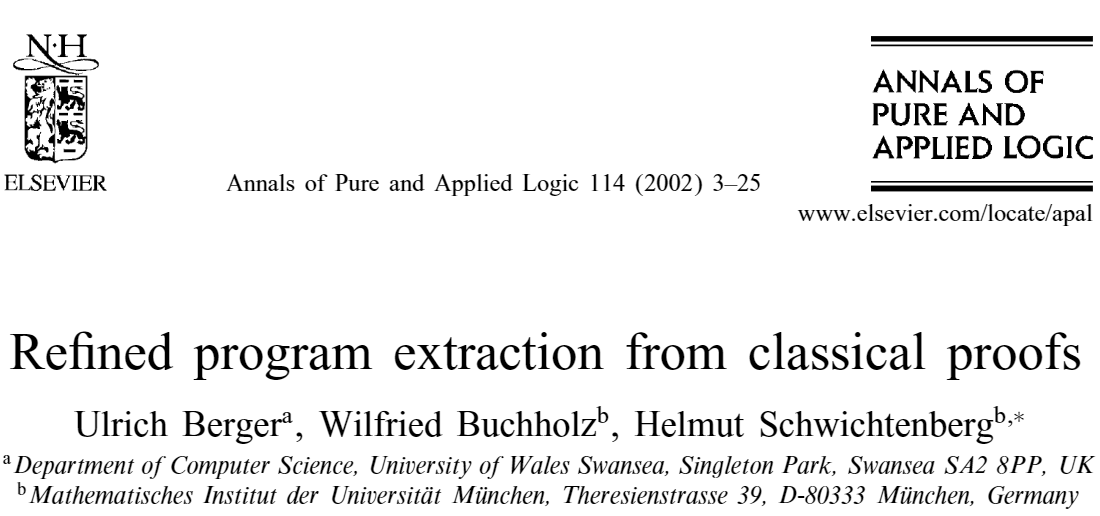
\includegraphics[width=\textwidth]{schwichtenberg.png}
			\end{subfigure}
		\vspace{.5cm}
			\begin{subfigure}[b]{0.49\textwidth}
				\centering
				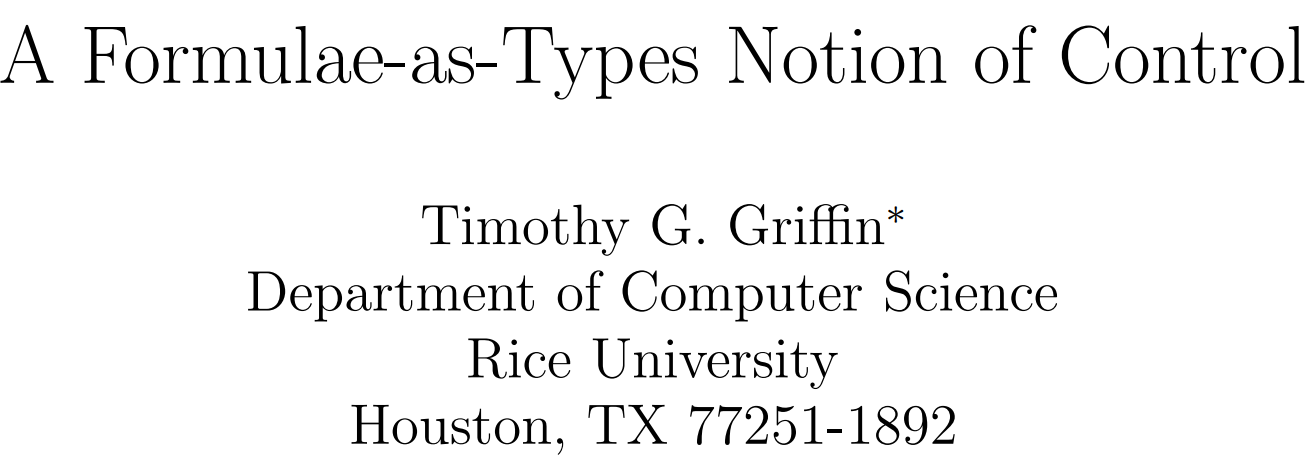
\includegraphics[width=\textwidth]{griffin.png}
			\end{subfigure}
			\begin{subfigure}[b]{0.49\textwidth}
				\centering
				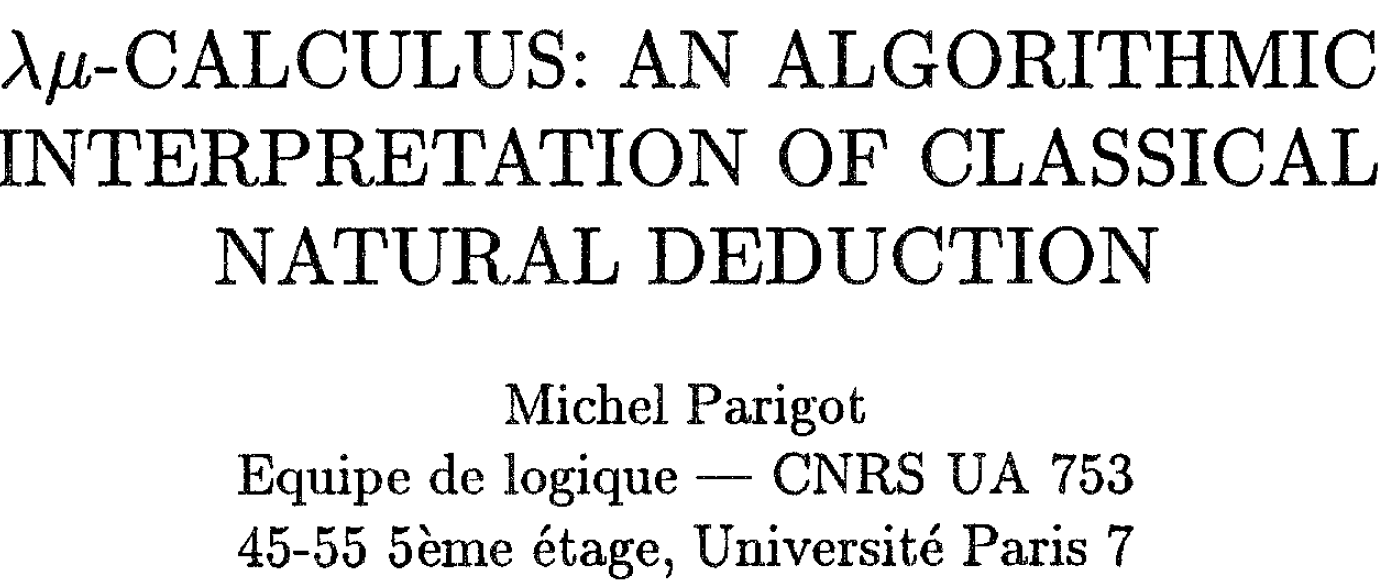
\includegraphics[width=0.9\textwidth]{parigot.png}
			\end{subfigure}
		\end{figure}
	\end{frame}
	
	\begin{frame}{Our approach}
		\begin{enumerate}
			\item Give an embedding of intuitionistic logic into classical logic.
			\item Leverage a classical prover to check the validity of the translated formula.
			\item Translate the generated proof/counter-example to one of the original formula.
		\end{enumerate}
	\end{frame}
	
	\section{The Embedding}
	
	\begin{frame}{Overview}
		\begin{enumerate}
			\item Tseytin-like Normalization
			\item Classical Encoding of Kripke Semantics
			\item Reduction of the Encoding
		\end{enumerate}
	\end{frame}

	\begin{frame}{Tseytin-like Normalization}
			\begin{lemma}[Tseytin-like Normalization, propositional case]
				Let $\varphi$ be a propositional formula. There is effectively a set $\mathcal S$ of formulas of the form $$(A\wedge B)\to C, A\to (B\wedge C), (A\vee B)\to C, A\to (B\vee C), (A\to B)\to C$$ and new propositional variable $P_\varphi$ such that $\varphi$ is valid if and only if $\mathcal S\to P_\varphi$ is.
			\end{lemma}	
	\end{frame}

	\begin{frame}{Example}
		For the non-intuitionistic tautology $\varphi = (A\to B)\vee (B\to A)$ we can have
		\begin{align*}
			\mathcal S &= \{\phantom{(P_{A\to B}\vee P_{B\to A})\to P_\varphi, (A\to B)\to P_{A\to B}, (B\to A)\to P_{B\to A}\}}
		\end{align*}
	\end{frame}

	\begin{frame}{Example}
		For the non-intuitionistic tautology $\varphi = (A\to B)\vee (B\to A)$ we can have
		\begin{align*}
			\mathcal S &= \{(P_{A\to B}\vee P_{B\to A})\to P_\varphi\phantom{, (A\to B)\to P_{A\to B}, (B\to A)\to P_{B\to A}\}}
		\end{align*}
	\end{frame}

	\begin{frame}{Example}
		For the non-intuitionistic tautology $\varphi = (A\to B)\vee (B\to A)$ we can have
		\begin{align*}
			\mathcal S &= \{(P_{A\to B}\vee P_{B\to A})\to P_\varphi, (A\to B)\to P_{A\to B}\phantom{, (B\to A)\to P_{B\to A}\}}
		\end{align*}
	\end{frame}

	\begin{frame}{Example}
		For the non-intuitionistic tautology $\varphi = (A\to B)\vee (B\to A)$ we can have
		\begin{align*}
			\mathcal S &= \{(P_{A\to B}\vee P_{B\to A})\to P_\varphi, (A\to B)\to P_{A\to B}, (B\to A)\to P_{B\to A}\phantom{\}}
		\end{align*}
	\end{frame}

	\begin{frame}{Example}
		For the non-intuitionistic tautology $\varphi = (A\to B)\vee (B\to A)$ we can have
		\begin{align*}
			\mathcal S &= \{(P_{A\to B}\vee P_{B\to A})\to P_\varphi, (A\to B)\to P_{A\to B}, (B\to A)\to P_{B\to A}\}
		\end{align*}
	\end{frame}
	
	\begin{frame}{Classical Encoding of Kripke Semantics - Propositional Case}
		Over a fixed propositional alphabet the theory of Kripke Frames is a first-order theory.
	\end{frame}
	
	\begin{frame}{Example}
		$$\bigwedge\{(P_{A\to B}\vee P_{B\to A})\to P_\varphi, (A\to B)\to P_{A\to B}, (B\to A)\to P_{B\to A}\} \to P_\varphi$$
		is intuitionistically valid iff
		$$\text{PO}(\preceq)\wedge\text{Persistent}\to \forall k\left(\bigwedge\left\{\substack{\forall u(k\preceq u\to (P_{A\to B}(u)\vee P_{B\to A}(u))\to P_\varphi(u)),\\ \forall u(k\preceq u\to \forall v(u\preceq v\to A(v)\to B(v))\to P_{A\to B}(u)),\\\forall u(k\preceq u\to \forall v(u\preceq v\to B(v)\to A(v))\to P_{B\to A}(u))}\right\} \to P_\varphi(k)\right)$$
		where PO$(\preceq)$ encodes that $\preceq$ is a partial order and Persistent persistency, e.g. $$\text{PO}(\preceq) = \forall u(u\preceq u)\wedge\forall u,v(u\preceq v\to v\preceq u)\wedge\forall u, v, w((u\preceq v\wedge v\preceq w)\to u\preceq w)$$
		$$\text{Persistent} = \bigwedge\{\forall u, v((u\preceq v\wedge P(u))\to P(v))\:|\:P\in\{A, B, P_{A\to B}, P_{B\to A}, P_\varphi\}\}$$
	\end{frame}
	
	\begin{frame}{Classical Encoding of Kripke Semantics - Predicate Case}
		We use a special predicate $E$ to encode that an element exists at a world.
		Now as in the predicate case we can encode the Kripke Semantics:
		\begin{align*}
			\varphi'= &\:\text{PartialOrder}(\preceq) \to \forall u \forall w (u\preceq w\to \text{DomainSubset}(u, w))\\
			&\to\forall u(\text{DomainClosed}(u))\to \forall u\forall w (u\preceq w\to \text{Persistent}(u, w))\\
			&\to \forall k(\mathcal S'\to P_\varphi(k))
		\end{align*}
	\end{frame}
	
	\begin{frame}{Reducing the Encoding - Propositional Case}
		Recall that we ended with the formula
		$$\text{PO}(\preceq)\wedge\text{Persistent}\to \forall k\left(\bigwedge\left\{\substack{\forall u(k\preceq u\to (P_{A\to B}(u)\vee P_{B\to A}(u))\to P_\varphi(u)),\\ \forall u(k\preceq u\to \forall v(u\preceq v\to A(v)\to B(v))\to P_{A\to B}(u)),\\\forall u(k\preceq u\to \forall v(u\preceq v\to B(v)\to A(v))\to P_{B\to A}(u))}\right\} \to P_\varphi(k)\right).$$
		Herbrandization:
		\[\phantom{\text{PO}(\preceq)\wedge\text{Persistent}\to \bigwedge\left\{\substack{\forall u({\color{red}s}\preceq u\to (P_{A\to B}(u)\vee P_{B\to A}(u))\to P_\varphi(u)),\\ \forall u({\color{red}s}\preceq u\to (u\preceq {\color{red}f_{A\to B}(u)}\to A({\color{red}f_{A\to B}(u)})\to B({\color{red}f_{A\to B}(u)}))\to P_{A\to B}(u)),\\\forall u({\color{red}s}\preceq u\to (u\preceq  {\color{red}f_{B\to A}(u)}\to B({\color{red}f_{B\to A}(u)})\to A({\color{red}f_{B\to A}(u)}))\to P_{B\to A}(u))}\right\} \to P_\varphi({\color{red}s}).}\]
	\end{frame}
	
	\begin{frame}{Reducing the Encoding - Propositional Case}
		Recall that we ended with the formula
		$$\text{PO}(\preceq)\wedge\text{Persistent}\to \forall k\left(\bigwedge\left\{\substack{\forall u(k\preceq u\to (P_{A\to B}(u)\vee P_{B\to A}(u))\to P_\varphi(u)),\\ \forall u(k\preceq u\to \forall v(u\preceq v\to A(v)\to B(v))\to P_{A\to B}(u)),\\\forall u(k\preceq u\to \forall v(u\preceq v\to B(v)\to A(v))\to P_{B\to A}(u))}\right\} \to P_\varphi(k)\right).$$
		Herbrandization:
			\[\text{PO}(\preceq)\wedge\text{Persistent}\to \bigwedge\left\{\substack{\forall u({\color{red}s}\preceq u\to (P_{A\to B}(u)\vee P_{B\to A}(u))\to P_\varphi(u)),\\ \forall u({\color{red}s}\preceq u\to (u\preceq {\color{red}f_{A\to B}(u)}\to A({\color{red}f_{A\to B}(u)})\to B({\color{red}f_{A\to B}(u)}))\to P_{A\to B}(u)),\\\forall u({\color{red}s}\preceq u\to (u\preceq  {\color{red}f_{B\to A}(u)}\to B({\color{red}f_{B\to A}(u)})\to A({\color{red}f_{B\to A}(u)}))\to P_{B\to A}(u))}\right\} \to P_\varphi({\color{red}s}).\]
	\end{frame}

	\begin{frame}{Reducing the Encoding - Propositional Case}
		$$\text{PO}(\preceq)\wedge\text{Persistent}\to \bigwedge\left\{\substack{\forall u({s}\preceq u\to (P_{A\to B}(u)\vee P_{B\to A}(u))\to P_\varphi(u)),\\ \forall u({s}\preceq u\to (u\preceq {f_{A\to B}(u)}\to A({f_{A\to B}(u)})\to B({f_{A\to B}(u)}))\to P_{A\to B}(u)),\\\forall u({s}\preceq u\to (u\preceq  {f_{B\to A}(u)}\to B({f_{B\to A}(u)})\to A({f_{B\to A}(u)}))\to P_{B\to A}(u))}\right\} \to P_\varphi({s}).$$
			We may assume $s$ is minimal and $f_{A\to B}, f_{B\to A}$ are non-decreasing:
			\begin{align*}
				&\phantom{\forall k(s\preceq k)\to\forall u(u\preceq f_{A\to B}(u))\to\forall u(u\preceq f_{B\to 	A}(u))\to\text{PO}(\preceq)\wedge\text{Persistent}}\\&\phantom{\to\bigwedge\left\{\substack{\forall u(P_{A\to B}(u)\vee P_{B\to A}(u))\to P_\varphi(u)),\\ \forall u(A(f_{A\to B}(u))\to B(f_{A\to B}(u)))\to P_{A\to B}(u)),\\\forall u((B(f_{B\to A}(u))\to A(f_{B\to A}(u)))\to P_{B\to A}(u))}\right\} \to P_\varphi(s)}.
			\end{align*}
	\end{frame}

	\begin{frame}{Reducing the Encoding - Propositional Case}
		$$\text{PO}(\preceq)\wedge\text{Persistent}\to \bigwedge\left\{\substack{\forall u({s}\preceq u\to (P_{A\to B}(u)\vee P_{B\to A}(u))\to P_\varphi(u)),\\ \forall u({s}\preceq u\to (u\preceq {f_{A\to B}(u)}\to A({f_{A\to B}(u)})\to B({f_{A\to B}(u)}))\to P_{A\to B}(u)),\\\forall u({s}\preceq u\to (u\preceq  {f_{B\to A}(u)}\to B({f_{B\to A}(u)})\to A({f_{B\to A}(u)}))\to P_{B\to A}(u))}\right\} \to P_\varphi({s}).$$
		We may assume $s$ is minimal and $f_{A\to B}, f_{B\to A}$ are non-decreasing:
		\begin{align*}
				&\forall k(s\preceq k)\to\forall u(u\preceq f_{A\to B}(u))\to\forall u(u\preceq f_{B\to A}(u))\to\text{PO}(\preceq)\wedge\text{Persistent}\\&\to\bigwedge\left\{\substack{\forall u(P_{A\to B}(u)\vee P_{B\to A}(u))\to P_\varphi(u)),\\ \forall u(A(f_{A\to B}(u))\to B(f_{A\to B}(u)))\to P_{A\to B}(u)),\\\forall u((B(f_{B\to A}(u))\to A(f_{B\to A}(u)))\to P_{B\to A}(u))}\right\} \to P_\varphi(s).
		\end{align*}
	\end{frame}

	\begin{frame}{Reducing the Encoding - Propositional Case}
		It is sufficient to consider structures $\mathcal M_T = (M_T, I_T)$ where:
		\begin{itemize}
			\item $M_T$ is the set of sequences without repetition on the newly introduced function symbols ($\{\epsilon, f_{A\to B}, f_{B\to A}, f_{A\to B}f_{B\to A}, f_{B\to A}f_{A\to B}\}$ in our case).
			\item $\preceq$ is interpreted as the prefix-order.
			\item $$f_\psi^{I_T}(f_1\dots f_n) = \begin{cases}
				f_1\dots f_n, &\text{if $f_\psi$ occurs in $f_1\dots f_n$,}\\
				f_1\dots f_nf_\psi, &\text{else.}			
			\end{cases}$$
		\end{itemize}
 	\end{frame}


	
	\begin{frame}{Reducing the Encoding - Propositional Case}
		In our example this corresponds to the following:
		\begin{figure}[width=0.9\textwidth]
			\begin{center}
				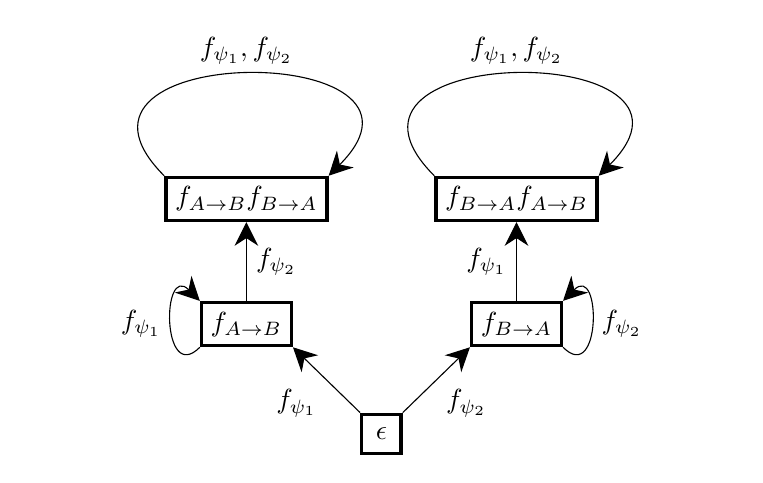
\begin{tikzpicture}[squarednode/.style={rectangle, draw, very thick, minimum size=5mm}]
					\node (center) {};
					\node[squarednode]      (right1)   [right=of center] {$f_{B\to A}$};
					\node[squarednode]      (right2)   [above=of right1] {$f_{B\to A}f_{A\to B}$};
					\node[squarednode]      (left1)    [left=of center] {$f_{A\to B}$};
					\node[squarednode]      (left2)    [above=of left1] {$f_{A\to B}f_{B\to A}$};
					\node[squarednode]      (lower)       	[below=of center] {$\epsilon$};
					\draw[-{Stealth[length=3mm, width=3mm]}] (lower.north west) -- (left1.south east) node [midway, below left] {$f_{\psi_1}$};
					\draw[-{Stealth[length=3mm, width=3mm]}] (lower.north east) -- (right1.south west) node [midway, below right] {$f_{\psi_2}$};
					\draw[-{Stealth[length=3mm, width=3mm]}] (left1.north) -- (left2.south) node [midway, right] {$f_{\psi_2}$};
					\draw[-{Stealth[length=3mm, width=3mm]}] (right1.north) -- (right2.south) node [midway, left] {$f_{\psi_1}$};
					\draw[-{Stealth[length=3mm, width=3mm]}] (left1.south west) to [out=225, in=135, loop, looseness=3] node [left] {$f_{\psi_1}$} (left1.north west);		
					\draw[-{Stealth[length=3mm, width=3mm]}] (right1.south east) to [out=315, in=45, loop, looseness=3] node [right] {$f_{\psi_2}$} (right1.north east);
					\draw[-{Stealth[length=3mm, width=3mm]}] (left2.north west) to [out=135, in=45, loop, looseness=3] node [midway, above] {$f_{\psi_1}, f_{\psi_2}$} (left2.north east);
					\draw[-{Stealth[length=3mm, width=3mm]}] (right2.north west) to [out=135, in=45, loop, looseness=3] node [midway, above] {$f_{\psi_1}, f_{\psi_2}$} (right2.north east);		
				\end{tikzpicture}
			\end{center}
		\end{figure}
	\end{frame}
	
	\begin{frame}{Reducing the Encoding - Propositional Case}
		And indeed there is a counter-model to $(A\to B)\vee (B\to A)$ with such a frame:
		\vspace{.5cm}
		\begin{figure}[width=0.9\textwidth]
			\begin{center}
				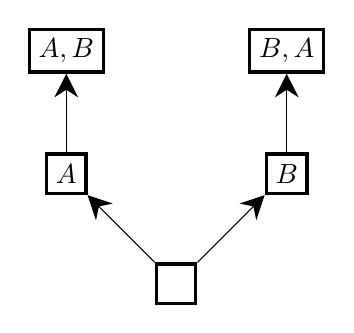
\begin{tikzpicture}[squarednode/.style={rectangle, draw, very thick, minimum size=5mm}]
					\node (center) {};
					\node[squarednode]      (right1)   [right=of center] {$B$};
					\node[squarednode]      (right2)   [above=of right1] {$B, A$};
					\node[squarednode]      (left1)    [left=of center] {$A$};
					\node[squarednode]      (left2)    [above=of left1] {$A, B$};
					\node[squarednode]      (lower)       	[below=of center] {$ $};
					\draw[-{Stealth[length=3mm, width=3mm]}] (lower.north west) -- (left1.south east) node [midway, below left] {};
					\draw[-{Stealth[length=3mm, width=3mm]}] (lower.north east) -- (right1.south west) node [midway, below right] {};
					\draw[-{Stealth[length=3mm, width=3mm]}] (left1.north) -- (left2.south) node [midway, right] {};
					\draw[-{Stealth[length=3mm, width=3mm]}] (right1.north) -- (right2.south) node [midway, left] {};
				\end{tikzpicture}
			\end{center}
		\end{figure}
	\end{frame}

	\begin{frame}{Reducing the Encoding - Propositional Case}
		\vspace*{-.5cm}
		\begin{align*}
			&\forall k(s\preceq k)\to\forall u(u\preceq f_{A\to B}(u))\to\forall u(u\preceq f_{B\to A}(u))\to\text{PO}(\preceq)\wedge\text{Persistent}\\&\to\bigwedge\left\{\substack{\forall u(P_{A\to B}(u)\vee P_{B\to A}(u))\to P_\varphi(u)),\\ \forall u(A(f_{A\to B}(u))\to B(f_{A\to B}(u)))\to P_{A\to B}(u)),\\\forall u((B(f_{B\to A}(u))\to A(f_{B\to A}(u)))\to P_{B\to A}(u))}\right\} \to P_\varphi(s).
		\end{align*}
		This allows us to eliminate the remaining quantifiers...
		\begin{align*}
			&\bigwedge\left\{P(u)\to P(v)\:|\:P\in\left\{\substack{A, B,\\P_{A\to B}, P_{B\to A}, P_\varphi}\right\}, (u, v)\in \left\{\substack{(\epsilon, f_{A\to B}), (\epsilon, f_{B\to A}),\\ (f_{A\to B}, f_{A\to B}f_{B\to A}), (f_{B\to A}, f_{B\to A}f_{A\to B})}\right\}\right\}\\&\to\bigwedge\left\{(P_{A\to B}(u)\to P_{B\to A}(u))\to P_\varphi(u)\:|\:u\in \{\epsilon, f_{A\to B}, f_{B\to A}, f_{A\to B}f_{B\to A}, f_{B\to A}f_{A\to B}\}\right\}\\& \to
			\bigwedge\left\{(A(v)\to B(v))\to P_{A\to B}(u)\:|\:(u, v)\in \left\{\substack{(\epsilon, f_{A\to B}), (f_{A\to B}, f_{A\to B}), (f_{A\to B}f_{B\to A}, f_{A\to B}f_{B\to A}),\\(f_{B\to A}, f_{B\to A}f_{A\to B}), (f_{B\to A}f_{A\to B}, f_{B\to A}f_{A\to B})}\right\}\right\}\\& \to
			\bigwedge\left\{(B(v)\to A(v))\to P_{B\to A}(u)\:|\:(u, v)\in \left\{\substack{(\epsilon, f_{B\to A}), (f_{B\to A}, f_{B\to A}), (f_{B\to A}f_{A\to B}, f_{B\to A}f_{A\to B}),\\(f_{A\to B}, f_{A\to B}f_{B\to A}), (f_{A\to B}f_{B\to A}, f_{A\to B}f_{B\to A})}\right\}\right\}\\&\to P_\varphi(\epsilon).
		\end{align*}
	\end{frame}
	
	\begin{frame}{Reducing the Encoding - Propositional Case}
		\begin{theorem}
			\label{thm:reduction-propositional}
			Let $\mathcal S$ be as on Slide 9 and $\mathcal F_\to\subseteq\mathcal S$ denote the subset of formulas of the form $(A\to B)\to C$ and $\Lambda$ denote the set of sequences without repetition over $\mathcal F_\to$. For each atom $A$ and $k\in\Lambda$ consider a new atom $A^k$. Obtain $\mathcal S^\#$ by including:
			\begin{itemize}
				\item $A^k\to A^{k\psi}$ for each atom $A$ occurring in $\mathcal S$, $k\in\Lambda$ and $\psi\in\mathcal F_\to$ not occurring in $k$.
				\item $A^k\to (B^k\circ C^k)$ for each $\circ\in\{\wedge,\vee\}$, $A\to (B\circ C)\in\mathcal S$, $k\in\Lambda$.
				\item $(A^k\circ B^k)\to C^k$ for each $\circ\in\{\wedge,\vee\}$, $A\to (B\circ C)\in\mathcal S$, $k\in\Lambda$.
				\item $(A^{k\psi}\to B^{k\psi})\to C^k$ for $\psi = (A\to B)\to C\in\mathcal S$, $k\in\Lambda$ if $\psi$ does not occur in $k$.
			\end{itemize}
			Then, $\bigwedge S\to P$ is intuitionistically valid iff $\bigwedge S^\#\to P^\epsilon$ is classically valid, where $\epsilon$ denotes the empty sequence.
		\end{theorem}
	\end{frame}
	
	\begin{frame}{Reducing the Encoding - Predicate Case}
		\begin{itemize}
			\item Essentially works the same, it is also possible to eliminate $\preceq$ and just consider models with the term algebra of newly introduced function symbols as domain.
			\item It is \textbf{not} possible to completely eliminate quantification over worlds as some sentences only have counter-models with an infinite number of worlds.
		\end{itemize}
	\end{frame}

	\section{Implementation}
	
	\begin{frame}{Implementation}
		\centering
		\begin{figure}
			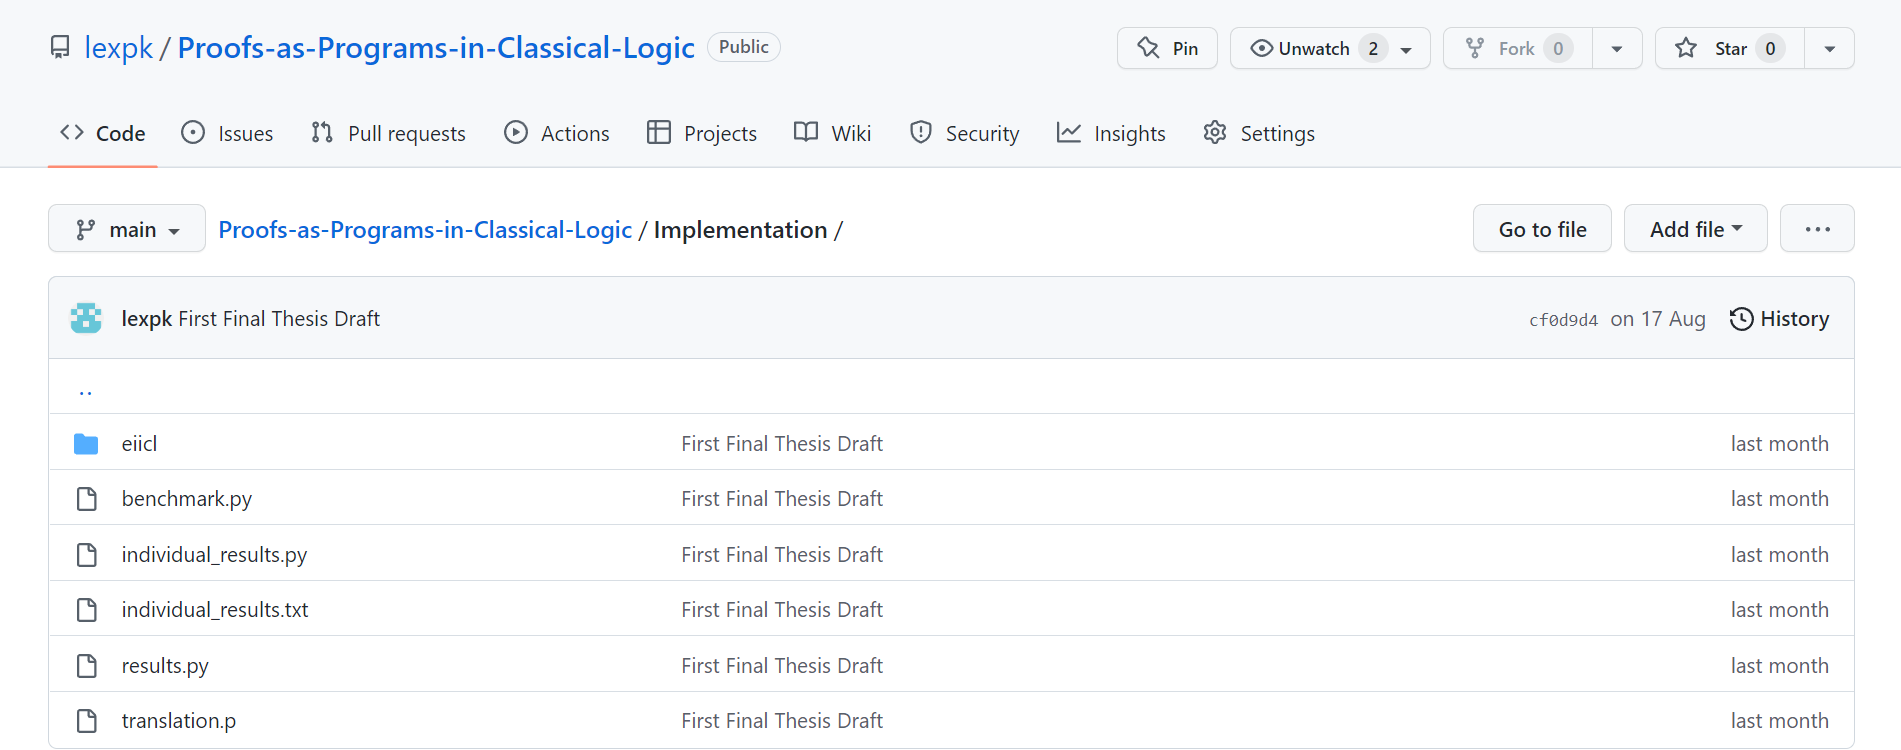
\includegraphics[width=\textwidth]{implementation.png}
		\end{figure}
		$\sim$3000 lines of rust code for the translation + $\sim$400 lines of python benchmarking
	\end{frame}


	\begin{frame}{Benchmark}
		\begin{figure}
				\begin{subfigure}{\textwidth}
					\scriptsize
					$$\begin{array}{*{13}c}
					&\text{AGT}&\text{ALG}&\text{COM}&\text{CSR}&\text{GEJ}&\text{GEO}&\text{GPJ}&\text{GRA}&\text{GRP}&\text{HAL}&\text{KRS}&\text{LCL}\\
					\text{Proven}&5&170&0&0&58&3&4&2&0&0&0&30\\
					\text{Disproven}&0&0&0&0&0&0&0&0&0&0&0&0\\
					\text{Timeout}&47&29&3&29&107&74&1&16&5&5&9&128
				\end{array}$$
				$$\begin{array}{*{13}c}
					&\text{MGT}&\text{MSC}&\text{NLP}&\text{NUM}&\text{PLA}&\text{PUZ}&\text{SET}&\text{SWC}&\text{SWV}&\text{SYJ}&\text{SYN}&\text{TOP}\\
					\text{Proven}&9&1&9&2&0&5&27&1&64&65&54&1\\
					\text{Disproven}&12&0&0&0&0&1&0&0&2&3&13&0\\
					\text{Timeout}&69&1&237&82&6&1&297&422&154&108&298&2
				\end{array}$$
				\end{subfigure}
				\begin{subfigure}{0.9\textwidth}
					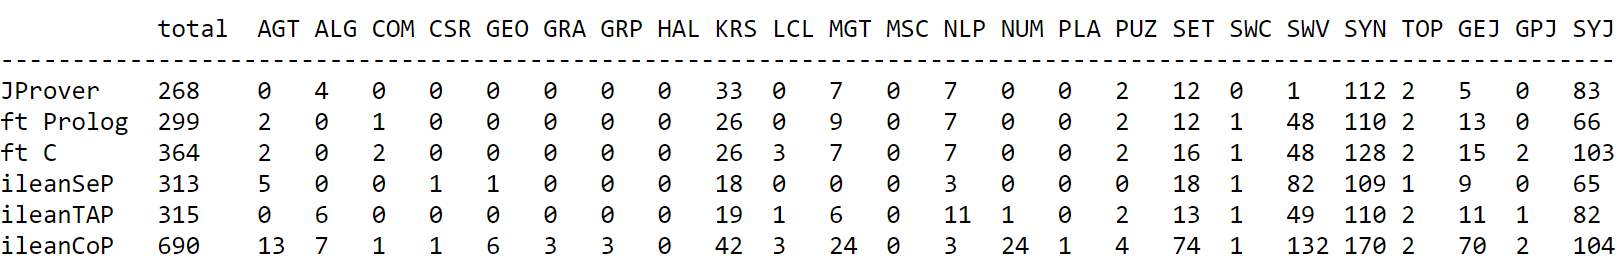
\includegraphics[width=\textwidth]{comparison.png}
					\caption{Comparison on different problem sections}
				\end{subfigure}
		\end{figure}
	\end{frame}
	
	\section{Conclusion and Outlook}
	
\begin{frame}[standout]
	\Huge\textsc{Thank You}
	
	\vfill
	
	\LARGE\textsc{Questions?}
\end{frame}
	
\end{document}